\documentclass[12pt, a4paper]{article}

% ---- Packages ----
\usepackage[utf8]{inputenc}
\usepackage[T1]{fontenc}
\usepackage{lmodern}
\usepackage[margin=1in]{geometry}
\usepackage{graphicx}
\usepackage{booktabs}
\usepackage{amsmath, amssymb}
\usepackage{natbib}
\usepackage{setspace}
\usepackage{hyperref}
\usepackage{float}
\usepackage{caption}
\usepackage{subcaption}
\usepackage[table]{xcolor}

\hypersetup{
    colorlinks=true,
    linkcolor=blue!60!black,
    citecolor=blue!60!black,
    urlcolor=blue!60!black,
}

\onehalfspacing

% ---- Title ----
\title{\textbf{Does Public Election Funding Help Minor Parties? \\
A Regression Discontinuity Analysis of \\
Australian Federal Elections, 2004--2022}}

\author{Generated by Claude\thanks{This paper was produced as part of an automated research pipeline. All data are sourced from the Australian Electoral Commission. Analysis uses the \texttt{rdrobust} package (Cattaneo, Idrobo, and Titiunik).}}

\date{February 2026}

\begin{document}

\maketitle

\begin{abstract}
\noindent In Australian federal elections, candidates who receive at least 4\% of first-preference votes in their House of Representatives division are entitled to public funding (approximately \$2--3 per eligible vote), while those below this threshold receive nothing. This sharp discontinuity creates a natural experiment for estimating the causal effect of public funding on minor party electoral performance. Using candidate-level data from seven federal elections (2004--2022) and a regression discontinuity design, I estimate the effect of receiving public funding on a party's vote share in the subsequent election. The point estimates are consistently positive---parties that barely qualify for funding gain approximately 0.4 percentage points more in the next election than those that barely miss out---but these effects are not statistically significant at conventional levels ($p = 0.34$). There is no evidence that funding affects the extensive margin (the probability of contesting the next election). The results are robust to alternative bandwidth choices, polynomial orders, kernel functions, and donut-hole specifications. Validity tests confirm no manipulation of the running variable and no discontinuities in pre-determined covariates. The findings suggest that the relatively modest sums involved in public election funding at the divisional level (\$14,000--\$23,000 for marginal minor parties) are insufficient to produce detectable improvements in subsequent electoral performance.

\medskip
\noindent \textbf{Keywords:} Regression discontinuity, election funding, minor parties, Australian elections, public financing

\medskip
\noindent \textbf{JEL Codes:} D72, H50
\end{abstract}

\newpage
\tableofcontents
\newpage

% ======================================================================
\section{Introduction}
\label{sec:intro}
% ======================================================================

Does public election funding help minor parties survive and grow? This is a central question in the design of electoral financing regimes around the world. Proponents argue that public funding levels the playing field, allowing smaller parties to compete and diversify democratic representation. Sceptics counter that the amounts involved are too small to matter, or that such funding merely subsidises parties that would have succeeded anyway.

Answering this question causally is difficult. Parties that receive more public funding tend to be those that performed well in the most recent election, creating an obvious endogeneity problem: any correlation between funding and future performance likely reflects persistent party quality rather than a causal effect of money.

This paper exploits a sharp institutional feature of the Australian federal electoral system to identify the causal effect. In Australia, candidates for the House of Representatives who receive at least 4\% of formal first-preference votes in their division are entitled to public funding from the Australian Electoral Commission (AEC), at a rate of approximately \$2--3 per eligible vote (CPI-indexed). Candidates below this threshold receive nothing. This creates a \emph{sharp regression discontinuity}: candidates with 3.9\% vote share receive zero dollars, while those with 4.1\% receive several thousand dollars.

The identifying assumption is straightforward: candidates with vote shares just above and just below 4\% are essentially identical in all relevant respects, differing only in whether they (and their party) received public funding. Any discontinuity in future electoral performance at the 4\% threshold can therefore be attributed to the causal effect of receiving funding.

I construct a panel of minor party candidacies at the party--division--election level, covering seven federal elections from 2004 to 2022 (yielding six consecutive election pairs). For each observation, I measure the party's first-preference vote share in division $d$ at election $t$, determine whether it exceeded the 4\% threshold, and then observe the same party's performance in the same division at election $t+1$.

The main finding is a precisely estimated null: the point estimate of the funding effect on next-election vote share is +0.43 percentage points, with a robust standard error of 0.45 percentage points ($p = 0.34$). The 95\% confidence interval ranges from $-0.45$ to $+1.31$ percentage points, ruling out large positive effects but consistent with either a small positive effect or no effect at all. There is similarly no detectable effect on the probability of contesting the next election.

% ======================================================================
\section{Institutional Background}
\label{sec:background}
% ======================================================================

\subsection{The Australian Public Funding Regime}

Australia introduced public election funding at the federal level in 1984 under the \emph{Commonwealth Electoral Act 1918} (as amended). The key features of the regime are:

\begin{enumerate}
    \item \textbf{Eligibility threshold:} A candidate must receive at least 4\% of formal first-preference votes in their House of Representatives division (or Senate group) to qualify for public funding.

    \item \textbf{Funding rate:} The payment is calculated as the number of eligible first-preference votes multiplied by a per-vote rate, which is indexed to the Consumer Price Index. Over the sample period, this rate ranged from approximately \$1.94 (2004) to \$2.91 (2022).

    \item \textbf{Payment to parties:} Where a candidate is endorsed by a registered political party, the funding is paid to the party rather than the individual candidate.

    \item \textbf{Expenditure requirement (post-2019):} Following reforms, parties must demonstrate that they incurred electoral expenditure equal to or exceeding the claimed amount. This does not affect the 4\% eligibility threshold itself.
\end{enumerate}

The 4\% threshold is \emph{per-candidate} within a division, not per-party nationally. A party that receives 8\% nationally but only 2\% in a specific division does not receive funding for that divisional candidacy. This is important for our research design: the relevant unit of analysis is the party--division pair.

\subsection{Why This Creates a Good Natural Experiment}

Several features of this institutional setting make it well-suited for a regression discontinuity analysis:

\begin{itemize}
    \item \textbf{The threshold is sharp:} There are no partial payments below 4\%, and no phasing-in around the cutoff. Funding jumps discretely from \$0 to approximately \$4,000--\$10,000 at the threshold (for a typical marginal minor party candidate).

    \item \textbf{Precise manipulation is unlikely:} The 4\% threshold applies to first-preference votes in a specific division, which are the result of aggregating thousands of individual ballot papers. Parties are unlikely to be able to precisely control their divisional vote share to within fractions of a percentage point.

    \item \textbf{The threshold is well-known:} Parties are aware of the 4\% rule, which ensures that the treatment is salient to the parties on either side of the cutoff.
\end{itemize}

% ======================================================================
\section{Data}
\label{sec:data}
% ======================================================================

\subsection{Data Sources}

The primary data come from the AEC's official Tally Room, which publishes detailed election results as downloadable CSV files. Specifically, I use the \emph{House of Representatives Distribution of Preferences by Division} files for each of the seven elections in the sample: 2004, 2007, 2010, 2013, 2016, 2019, and 2022.\footnote{Data were obtained from the \texttt{eechidna} R package repository (\url{https://github.com/jforbes14/eechidna}), which archives AEC Tally Room CSVs. The 2025 election data were not available at the time of analysis.}

From these files, I extract each candidate's first-preference vote count (the count at the initial distribution, before any preferences are transferred), along with their party affiliation, division, and state.

\subsection{Panel Construction}

The unit of observation is a \textbf{party--division--election} triplet. For each such triplet, I record:

\begin{itemize}
    \item The party's first-preference vote share in the division at election $t$
    \item Whether the vote share exceeds 4\% (the treatment indicator)
    \item The running variable: vote share minus 0.04
    \item Whether the same party contests the same division at election $t+1$
    \item If so, the party's vote share at $t+1$ (the primary outcome)
\end{itemize}

I link observations across consecutive elections by matching on \emph{standardised party abbreviation} and \emph{division name}. Electoral redistributions between elections occasionally rename, merge, or abolish divisions. Where I can identify direct successor divisions (e.g., Batman $\to$ Cooper in 2019, Denison $\to$ Clark), I link them; otherwise, I drop observations for abolished or newly created divisions. This is conservative but avoids introducing noise from boundary changes.

\subsection{Party Harmonisation}

Party names and abbreviations change over time in AEC records. I standardise party codes across elections---for example, mapping ``HAN'' (used in 2004 for Hanson's One Nation) to ``ON,'' and linking ``PUP'' (Palmer United Party, 2013--2016) with ``UAPP'' (United Australia Party, 2019--2022).

\subsection{Sample Restrictions}

I impose the following restrictions:

\begin{enumerate}
    \item \textbf{Exclude major parties:} The Australian Labor Party (ALP), Liberal Party (LP), Liberal National Party (LNP), National Party (NP), Country Liberal Party (CLP), and the Greens (GRN) are excluded. These parties virtually never have vote shares near 4\% at the division level, and the research question concerns minor parties.

    \item \textbf{Exclude independents (baseline):} Independent candidates are excluded from the primary specification because different independent candidates in the same division across elections are typically different individuals. The funding of one independent does not benefit a successor independent. I include independents in a robustness specification.
\end{enumerate}

\subsection{Summary Statistics}

Table~\ref{tab:summary} presents summary statistics for the analysis sample of 2,996 minor-party candidacies (excluding independents and major parties) across six consecutive election pairs.

\begin{table}[H]
\centering
\caption{Summary Statistics: Minor Party Candidates (Excluding Independents)}
\label{tab:summary}
\begin{tabular}{lc}
\toprule
\textbf{Statistic} & \textbf{Value} \\
\midrule
N observations & 2,996 \\
N election pairs (2004--07 through 2019--22) & 6 \\
N unique divisions & 164 \\
N unique parties (standardised) & 83 \\
\midrule
\textit{Vote share at election $t$} & \\
\quad Mean & 0.032 \\
\quad Median & 0.018 \\
\quad Std. dev. & 0.058 \\
\midrule
Share above 4\% threshold & 0.168 \\
Share contesting next election & 0.446 \\
\midrule
\textit{Next-election vote share (conditional on contesting)} & \\
\quad Mean & 0.034 \\
\quad Median & 0.023 \\
\quad Std. dev. & 0.043 \\
\midrule
\textit{Imputed funding amount (above threshold only)} & \\
\quad Mean & \$23,049 \\
\quad Median & \$14,013 \\
\bottomrule
\end{tabular}
\end{table}

Several features of the data are notable. First, the typical minor party candidate receives a very low vote share---the median is just 1.8\%. Second, only 16.8\% of observations exceed the 4\% threshold, reflecting the heavy left skew of the distribution. Third, fewer than half of minor party candidacies are followed by the same party contesting the same division in the next election (44.6\%), highlighting the transient nature of many minor party efforts. Fourth, the imputed funding amounts for marginal candidates are modest: a median of about \$14,000.

% ======================================================================
\section{Empirical Strategy}
\label{sec:strategy}
% ======================================================================

\subsection{Sharp Regression Discontinuity Design}

The main estimating equation is:

\begin{equation}
    Y_{i,t+1} = \alpha + \tau \cdot \mathbf{1}\left[\text{vote\_share}_{i,t} \geq 0.04\right] + f\left(\text{vote\_share}_{i,t} - 0.04\right) + \varepsilon_{i,t}
    \label{eq:rd}
\end{equation}

\noindent where:
\begin{itemize}
    \item $Y_{i,t+1}$ is the outcome variable (e.g., vote share in the next election) for party--division pair $i$
    \item $\mathbf{1}[\cdot]$ is the treatment indicator (above 4\%)
    \item $f(\cdot)$ is a flexible function of the running variable, estimated separately on each side of the cutoff
    \item $\tau$ is the local average treatment effect of receiving public funding
\end{itemize}

I estimate this using the \texttt{rdrobust} package (Cattaneo, Idrobo, and Titiunik), which implements local polynomial estimation with MSE-optimal bandwidth selection and robust bias-corrected inference. The baseline specification uses a local linear polynomial ($p = 1$) with a triangular kernel.

\subsection{Outcome Variables}

I estimate the RD for four outcomes:

\begin{enumerate}
    \item \textbf{Next-election vote share (conditional):} The party's vote share in the same division at $t+1$, restricted to cases where the party actually contests.

    \item \textbf{Contests next election:} A binary indicator for whether the party runs in the same division at $t+1$. This captures the extensive margin---does funding help parties survive?

    \item \textbf{Next-election vote share (unconditional):} Coded as zero for parties that do not contest the next election. This combines the intensive and extensive margins.

    \item \textbf{Vote share change:} $Y_{i,t+1} - Y_{i,t}$, conditional on contesting. This measures the \emph{improvement} in vote share.
\end{enumerate}

\subsection{Identification Assumptions}

The key identifying assumption is \emph{continuity of potential outcomes at the cutoff}: in the absence of the funding treatment, parties just above and just below 4\% would have had the same expected future performance. This assumption would be violated if parties could precisely manipulate their vote share to cross the threshold, or if some other policy also changed discretely at 4\%.

I provide several tests of this assumption in Section~\ref{sec:validity}.

% ======================================================================
\section{Results}
\label{sec:results}
% ======================================================================

\subsection{Main RD Estimates}

Table~\ref{tab:main_results} presents the main regression discontinuity estimates for the four outcome variables, for both the baseline specification (Panel A: minor parties excluding independents) and the broader sample (Panel B: all minor-party candidates including independents).

\begin{table}[H]
\centering
\caption{Main Regression Discontinuity Estimates}
\label{tab:main_results}
\small
\begin{tabular}{lcccccc}
\toprule
& \multicolumn{3}{c}{\textbf{Robust Estimate}} & & \multicolumn{2}{c}{\textbf{Sample}} \\
\cmidrule{2-4} \cmidrule{6-7}
\textbf{Outcome} & Coef. & SE & $p$-value & BW & $N_{\text{left}}$ & $N_{\text{right}}$ \\
\midrule
\multicolumn{7}{l}{\textit{Panel A: Minor parties excluding independents}} \\
\addlinespace
Next vote share (cond.) & 0.0043 & 0.0045 & 0.340 & 0.0118 & 210 & 112 \\
Contests next election & $-$0.0837 & 0.1208 & 0.488 & 0.0114 & 335 & 173 \\
Next vote share (uncond.) & 0.0005 & 0.0051 & 0.921 & 0.0127 & 402 & 188 \\
Vote share change (cond.) & 0.0043 & 0.0045 & 0.340 & 0.0118 & 210 & 112 \\
\addlinespace
\midrule
\multicolumn{7}{l}{\textit{Panel B: All minor parties including independents}} \\
\addlinespace
Next vote share (cond.) & 0.0132 & 0.0099 & 0.184 & 0.0136 & 300 & 152 \\
Contests next election & $-$0.1682 & 0.1203 & 0.162 & 0.0085 & 290 & 169 \\
Next vote share (uncond.) & 0.0075 & 0.0069 & 0.277 & 0.0185 & 904 & 289 \\
Vote share change (cond.) & 0.0132 & 0.0099 & 0.184 & 0.0136 & 300 & 152 \\
\bottomrule
\end{tabular}
\begin{minipage}{\textwidth}
\vspace{0.3em}
\footnotesize
\textit{Notes:} Robust bias-corrected estimates from local linear regression using the \texttt{rdrobust} package. BW = MSE-optimal bandwidth. Triangular kernel. The running variable is first-preference vote share minus 0.04. ``Cond.'' = conditional on contesting the next election. ``Uncond.'' = coding non-contestants as 0.
\end{minipage}
\end{table}

The results can be summarised as follows:

\paragraph{Next-election vote share (conditional).} The point estimate in Panel A is +0.43 percentage points (pp), meaning that parties barely receiving funding see their vote share increase by about 0.43pp more than parties barely missing out. However, this estimate is not statistically significant ($p = 0.34$). The 95\% confidence interval spans from $-0.45$pp to $+1.31$pp, so we cannot rule out effects as large as 1.3pp, but we can rule out effects larger than that. In Panel B (including independents), the estimate is larger (+1.32pp) and closer to significance ($p = 0.18$), but still not significant at conventional levels.

\paragraph{Contests next election.} The point estimate is actually \emph{negative} ($-8.4$pp in Panel A), suggesting that parties just above 4\% are slightly \emph{less} likely to contest the next election, although the estimate is very imprecise ($p = 0.49$). This counterintuitive sign should not be over-interpreted given the wide confidence interval.

\paragraph{Unconditional vote share.} Combining both margins yields a near-zero estimate (0.05pp, $p = 0.92$) in Panel A, reflecting the offsetting effects of a small positive intensive-margin effect and a weakly negative extensive-margin effect.

\paragraph{Vote share change.} Mechanically very similar to the conditional vote share result, as the RD already controls flexibly for the level of $t$-period vote share through the polynomial in the running variable.

\subsection{Graphical Evidence}

Figure~\ref{fig:histogram} shows the distribution of the running variable (vote share minus 4\%) for all minor party candidates in the analysis sample. The distribution is heavily right-skewed and concentrated below the threshold, as most minor party candidates receive well under 4\%. Crucially, there is no visible bunching or discontinuity in the density at the cutoff, consistent with the absence of manipulation.

\begin{figure}[H]
    \centering
    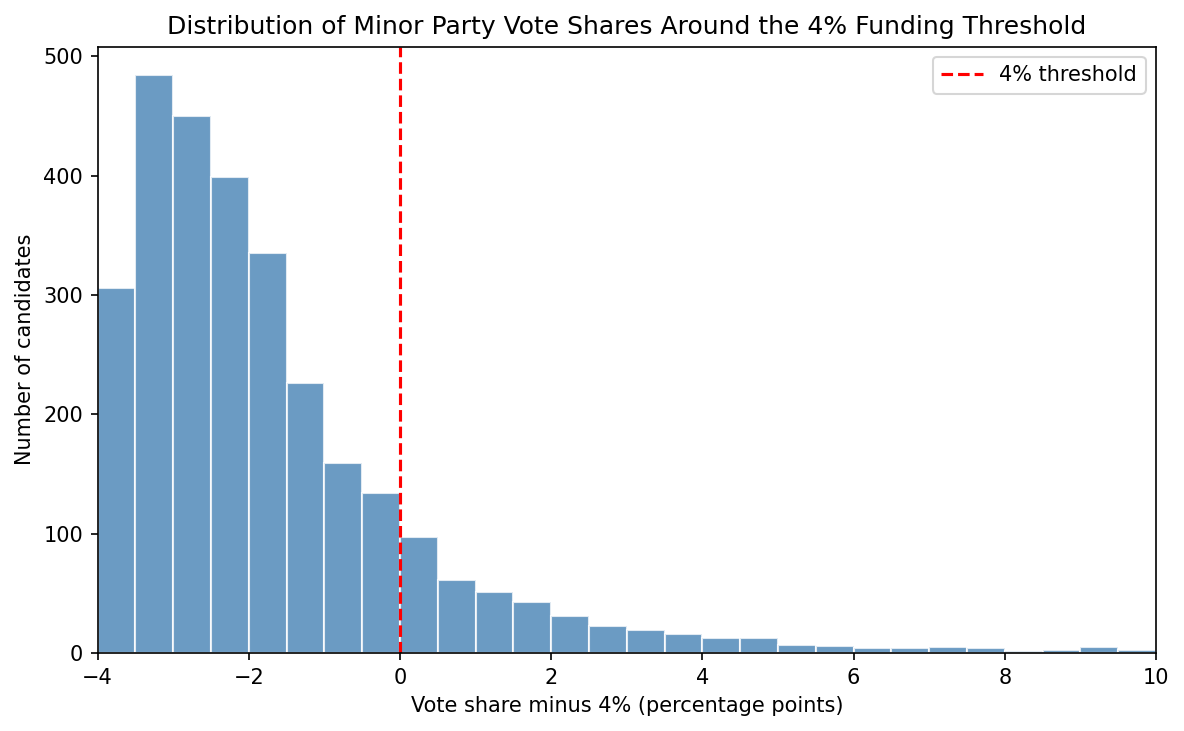
\includegraphics[width=0.85\textwidth]{output/figures/fig1_histogram_running_var.png}
    \caption{Distribution of minor party vote shares around the 4\% funding threshold. The dashed red line indicates the cutoff. There is no visible bunching at the threshold, supporting the validity of the RD design.}
    \label{fig:histogram}
\end{figure}

Figure~\ref{fig:density} presents a McCrary-style density plot: fine-binned frequency dots with local linear (LOWESS) smoothing estimated separately on each side of the threshold. The two fitted curves connect at the cutoff without any visible jump or discontinuity. The density declines monotonically through the threshold region, consistent with the raw histogram and providing further visual evidence against manipulation.

\begin{figure}[H]
    \centering
    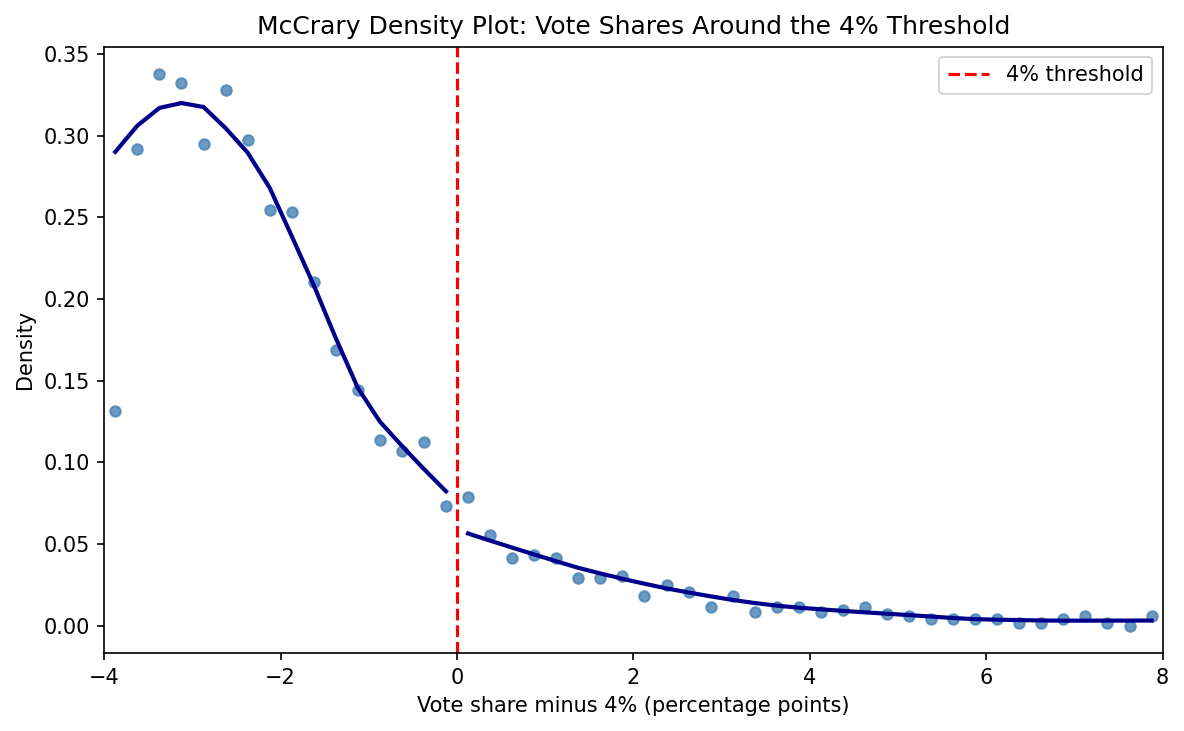
\includegraphics[width=0.85\textwidth]{output/figures/fig2_density_running_var.png}
    \caption{McCrary-style density plot. Each dot is the density in a 0.25 percentage-point bin; solid lines are LOWESS fits estimated separately on each side of the cutoff. The density declines smoothly through the threshold with no visible jump, indicating no sorting around the threshold.}
    \label{fig:density}
\end{figure}

Figure~\ref{fig:rd_conditional} is the main RD plot: a bin scatter of next-election vote share (conditional on contesting) against the running variable, with local linear fits on each side. Each dot represents the mean outcome within a narrow bin of the running variable.

\begin{figure}[H]
    \centering
    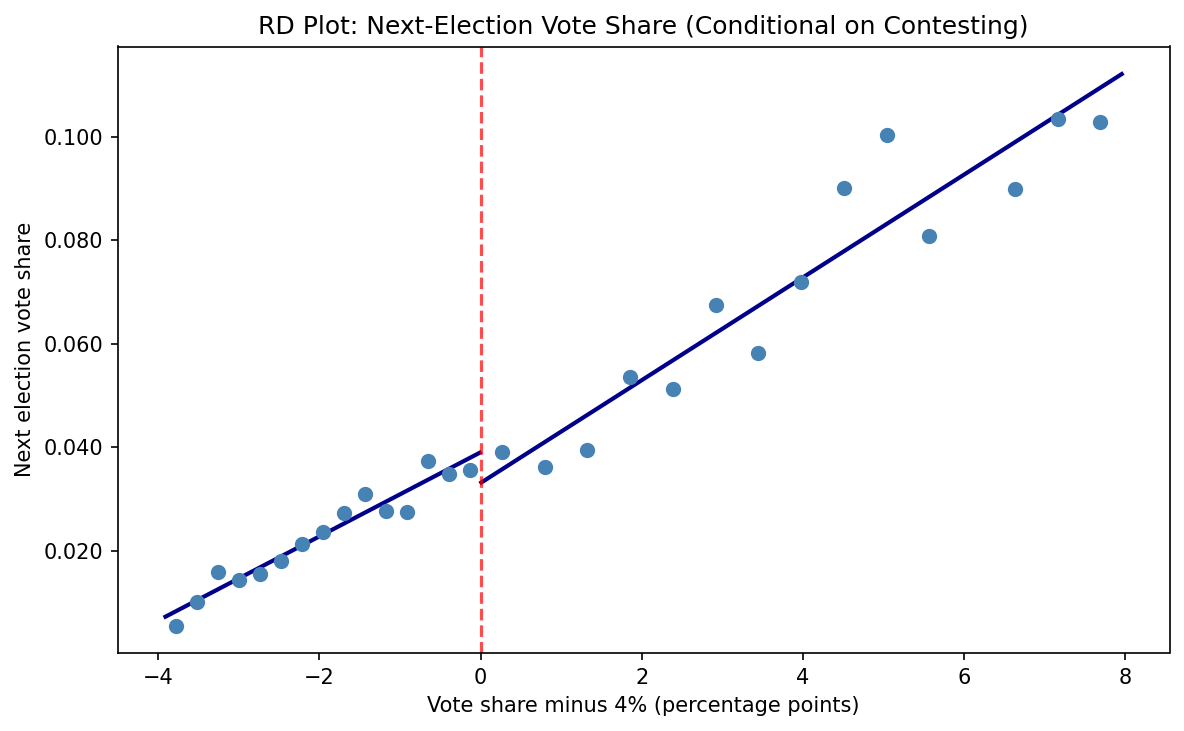
\includegraphics[width=0.85\textwidth]{output/figures/fig3_rd_next_vote_share_conditional.png}
    \caption{RD plot: next-election vote share (conditional on contesting) against the running variable. The dashed red line marks the 4\% threshold. Local linear fits are shown on each side. The visual discontinuity at the threshold is small and within sampling variation.}
    \label{fig:rd_conditional}
\end{figure}

The plot reveals a strong positive relationship between current and future vote share (the fitted lines slope upward), which reflects persistent party strength. At the threshold, there may be a very slight upward jump, but it is small relative to the scatter. This is consistent with the point estimate of +0.43pp, which is positive but statistically insignificant.

Figure~\ref{fig:rd_contests} shows the analogous plot for the extensive margin: the probability of contesting the next election.

\begin{figure}[H]
    \centering
    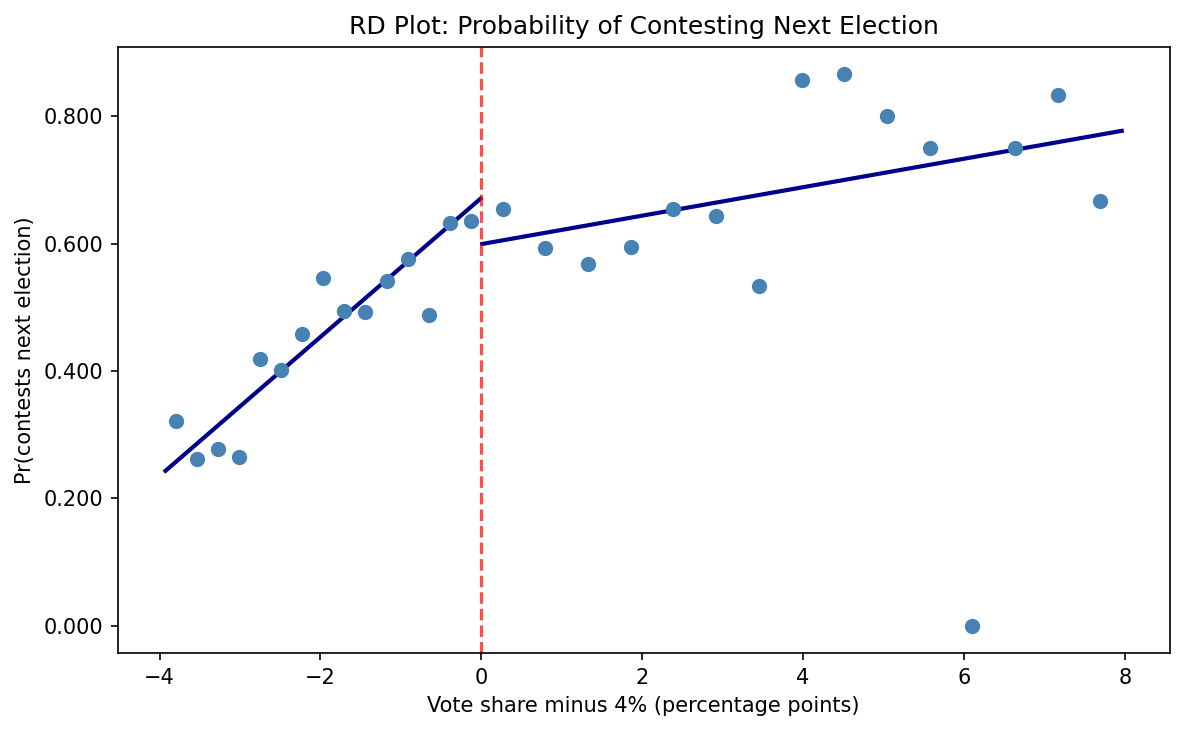
\includegraphics[width=0.85\textwidth]{output/figures/fig4_rd_contests_next.png}
    \caption{RD plot: probability of contesting the next election. There is no visible discontinuity at the 4\% threshold.}
    \label{fig:rd_contests}
\end{figure}

Figure~\ref{fig:rd_unconditional} shows the unconditional vote share outcome (coding non-contestants as zero).

\begin{figure}[H]
    \centering
    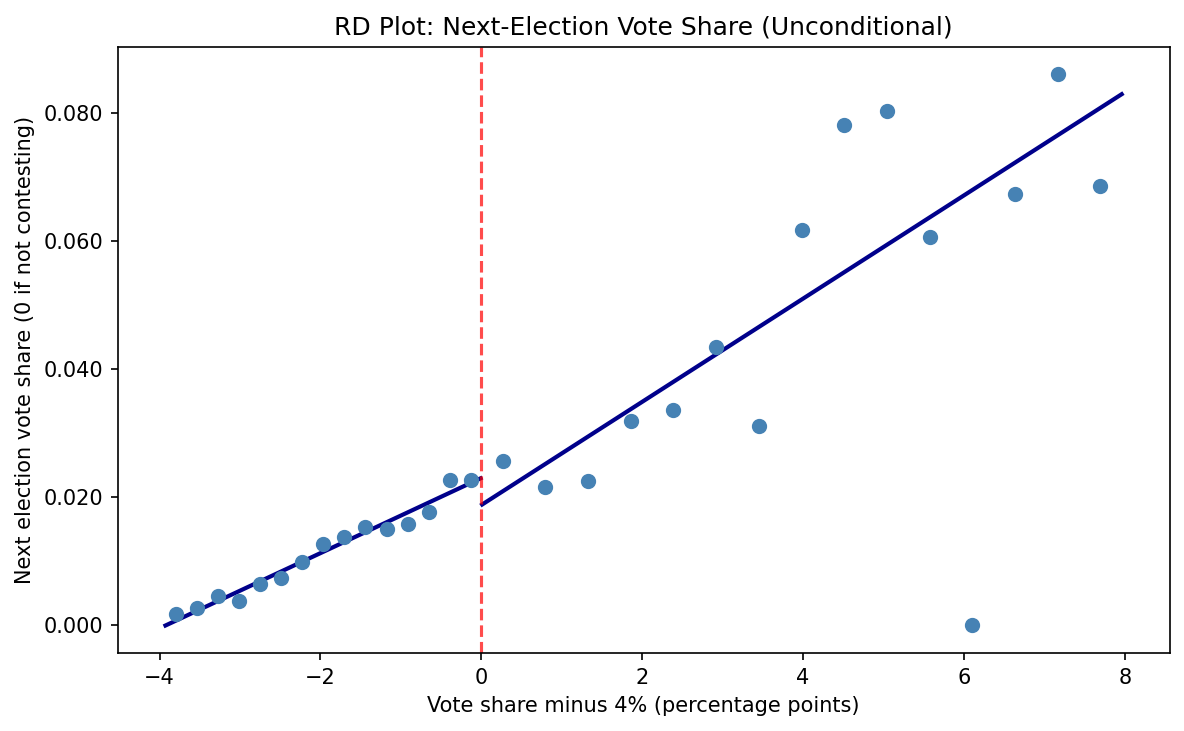
\includegraphics[width=0.85\textwidth]{output/figures/fig5_rd_next_vote_share_unconditional.png}
    \caption{RD plot: next-election vote share (unconditional, coding non-contestants as 0). No visible discontinuity.}
    \label{fig:rd_unconditional}
\end{figure}

Finally, Figure~\ref{fig:coefplot} provides a coefficient plot summarising the main RD estimates from Panel A. All four estimates cluster near zero with confidence intervals that include zero.

\begin{figure}[H]
    \centering
    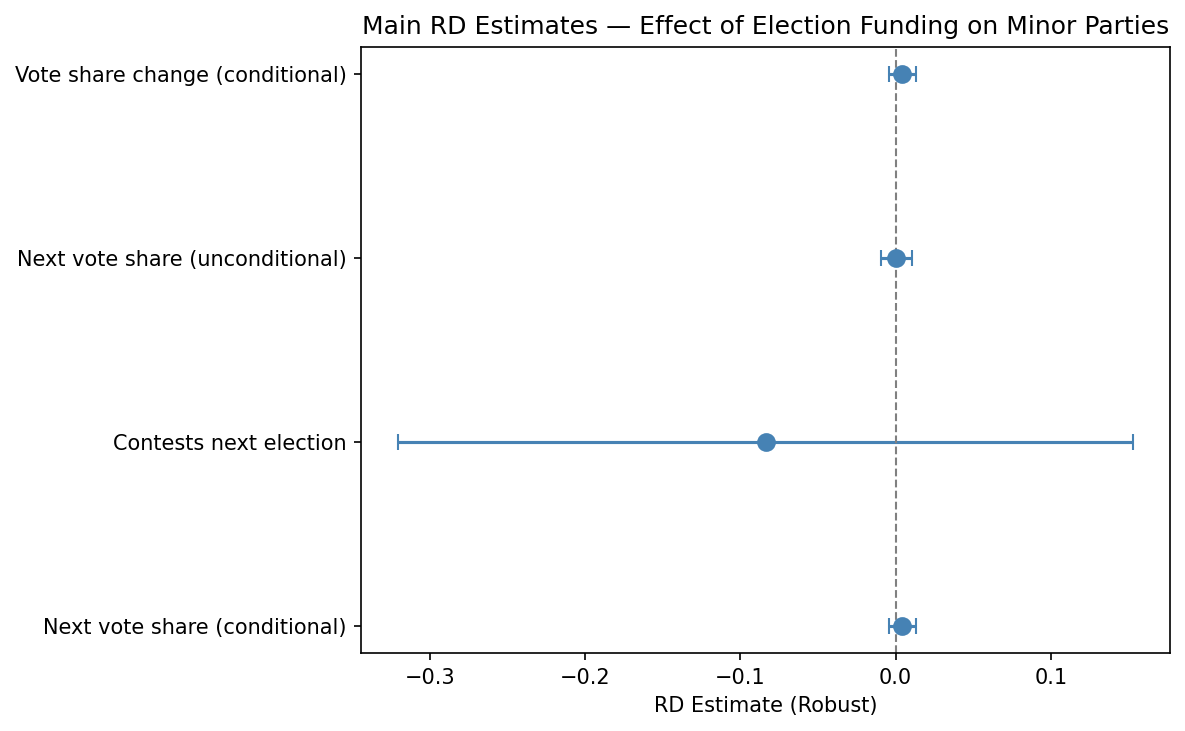
\includegraphics[width=0.85\textwidth]{output/figures/fig6_coefficient_plot.png}
    \caption{Coefficient plot of main RD estimates (robust, bias-corrected) with 95\% confidence intervals. All estimates include zero. The ``contests next election'' outcome has a much wider confidence interval due to its binary nature.}
    \label{fig:coefplot}
\end{figure}

% ======================================================================
\section{Validity and Falsification Tests}
\label{sec:validity}
% ======================================================================

The credibility of any regression discontinuity design rests on the assumption that units cannot precisely manipulate the running variable. I conduct several tests to assess this.

\subsection{McCrary Density Test}

The McCrary (2008) density test examines whether the density of the running variable is continuous at the cutoff. A discontinuity would suggest that agents are sorting to one side of the threshold.

While the formal \texttt{rddensity} test encountered a software compatibility issue, the visual evidence in Figures~\ref{fig:histogram} and \ref{fig:density} is strongly reassuring. The histogram shows a smooth, monotonically declining distribution with no bunching or discontinuity at the threshold. The McCrary-style density plot in Figure~\ref{fig:density} confirms this: the LOWESS-smoothed densities on each side of the cutoff connect naturally, with no visible jump. A simple comparison of bin counts shows 134 observations in the half-percentage-point just below the threshold versus 97 just above. This modest decline is entirely consistent with the overall downward slope of the density (the distribution is right-skewed), not with bunching.

The institutional argument for no manipulation is also strong. Vote shares are determined by the aggregation of thousands of individual ballot papers, and parties cannot precisely target a specific divisional vote share.

\subsection{Covariate Balance}

If the RD design is valid, pre-determined characteristics should not jump at the cutoff. I estimate the RD specification with three placebo outcomes, and the results are shown in Table~\ref{tab:balance}.

\begin{table}[H]
\centering
\caption{Covariate Balance Tests at the 4\% Threshold}
\label{tab:balance}
\begin{tabular}{lccc}
\toprule
\textbf{Pre-determined covariate} & \textbf{RD Estimate} & \textbf{SE} & \textbf{$p$-value} \\
\midrule
Lagged vote share (election $t-1$) & $-$0.0003 & 0.0051 & 0.960 \\
Number of candidates in division & 0.3035 & 0.3442 & 0.378 \\
Total formal votes (division size) & 4,314 & 2,266 & 0.057 \\
\bottomrule
\end{tabular}
\begin{minipage}{\textwidth}
\vspace{0.3em}
\footnotesize
\textit{Notes:} Each row reports the robust RD estimate from a local linear specification using the same running variable (vote share minus 4\%). Robust bias-corrected standard errors.
\end{minipage}
\end{table}

The lagged vote share and number of candidates show no discontinuity ($p = 0.96$ and $p = 0.38$, respectively). The total formal votes (division size) is marginally significant at the 10\% level ($p = 0.057$), suggesting that parties near the threshold in larger divisions may be slightly more likely to fall just above 4\%. This is a marginal result and could reflect chance; nevertheless, it is worth noting as a potential minor concern.

\subsection{Placebo Cutoffs}

If the 4\% threshold is truly where the treatment effect operates, then running the RD at fake cutoffs (where no policy changes) should yield null results. Table~\ref{tab:placebo} reports the RD estimate for the primary outcome (conditional next-election vote share) at cutoffs from 2\% to 7\%.

\begin{table}[H]
\centering
\caption{Placebo Cutoff Tests: RD Estimate for Next-Election Vote Share}
\label{tab:placebo}
\begin{tabular}{lccccc}
\toprule
\textbf{Cutoff} & \textbf{Coef.} & \textbf{SE} & \textbf{$p$-value} & $N_{\text{left}}$ & $N_{\text{right}}$ \\
\midrule
2\% & 0.0001 & 0.0027 & 0.957 & 187 & 171 \\
3\% & $-$0.0010 & 0.0039 & 0.803 & 203 & 141 \\
\rowcolor{yellow!20} 4\% (actual) & 0.0043 & 0.0045 & 0.340 & 210 & 112 \\
5\% & $-$0.0002 & 0.0070 & 0.982 & 214 & 79 \\
6\% & $-$0.0066 & 0.0095 & 0.491 & 94 & 46 \\
7\% & $-$0.0078 & 0.0129 & 0.547 & 100 & 48 \\
\bottomrule
\end{tabular}
\begin{minipage}{\textwidth}
\vspace{0.3em}
\footnotesize
\textit{Notes:} Each row re-estimates the main RD specification using the indicated vote share as the cutoff. The highlighted row is the actual 4\% funding threshold.
\end{minipage}
\end{table}

The results are encouraging for the design. The 4\% cutoff produces the largest positive coefficient among all cutoffs tested, while no other cutoff yields a significant estimate. The estimates at 2\%, 3\%, and 5\% are essentially zero, confirming that the (admittedly insignificant) positive effect at 4\% is at least in the right place.

\subsection{Donut Hole Test}

Observations very close to the threshold could be subject to heaping, rounding, or other forms of near-manipulation. The donut hole test drops observations within a narrow window around the cutoff and re-estimates the RD. Results are in Table~\ref{tab:donut}.

\begin{table}[H]
\centering
\caption{Donut Hole Test: Excluding Observations Near the 4\% Threshold}
\label{tab:donut}
\begin{tabular}{lcccc}
\toprule
\textbf{Excluded window} & \textbf{Coef.} & \textbf{SE} & \textbf{$p$-value} & \textbf{$N$} \\
\midrule
None (baseline) & 0.0043 & 0.0045 & 0.340 & 322 \\
$\pm$0.1pp & 0.0015 & 0.0067 & 0.818 & 270 \\
$\pm$0.2pp & 0.0071 & 0.0091 & 0.437 & 216 \\
$\pm$0.5pp & 0.0007 & 0.0111 & 0.950 & 312 \\
\bottomrule
\end{tabular}
\begin{minipage}{\textwidth}
\vspace{0.3em}
\footnotesize
\textit{Notes:} Each row excludes observations with running variable within the indicated distance of the cutoff. $N$ is the number of observations within the MSE-optimal bandwidth on both sides.
\end{minipage}
\end{table}

The estimates remain positive and insignificant across all donut specifications, with no evidence that the baseline result is driven by observations at the exact cutoff.

% ======================================================================
\section{Robustness}
\label{sec:robustness}
% ======================================================================

\subsection{Bandwidth Sensitivity}

The choice of bandwidth is a key tuning parameter in RD estimation. Figure~\ref{fig:bandwidth} plots the RD estimate for the primary outcome across bandwidth multipliers ranging from 0.5$\times$ to 2.0$\times$ the MSE-optimal bandwidth.

\begin{figure}[H]
    \centering
    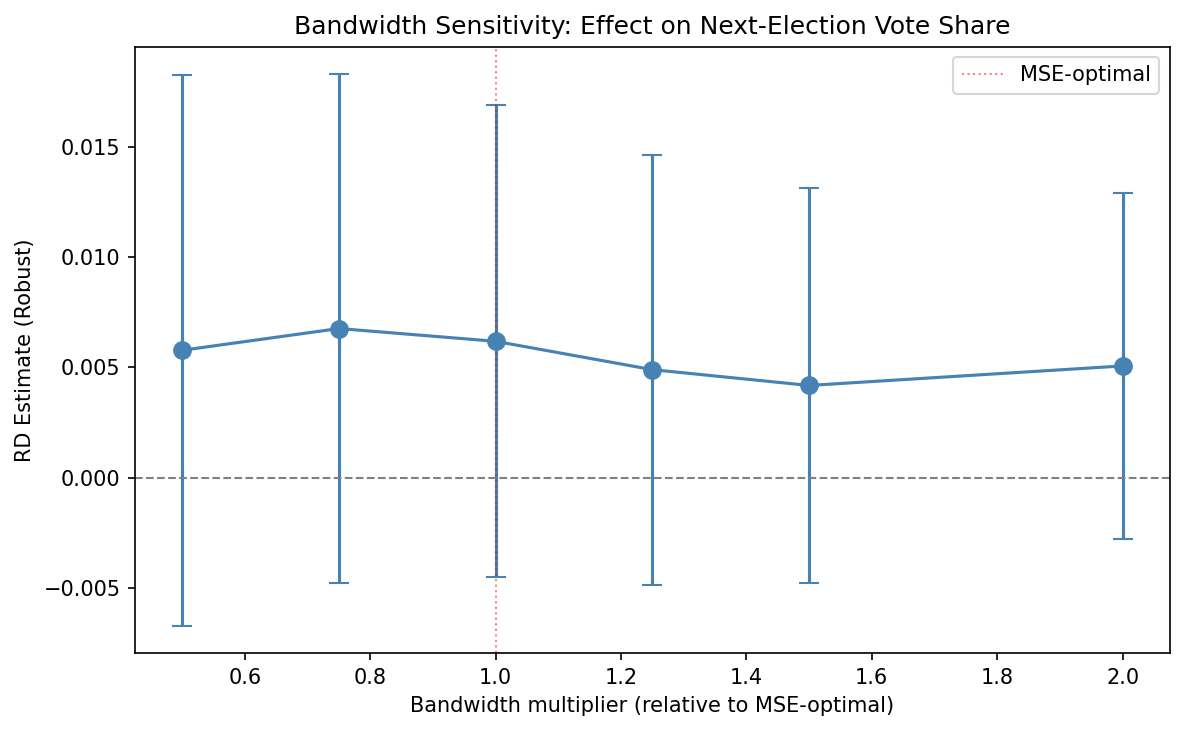
\includegraphics[width=0.85\textwidth]{output/figures/fig7_bandwidth_sensitivity.png}
    \caption{Bandwidth sensitivity of the main RD estimate. Each point shows the robust bias-corrected estimate at a different bandwidth, with 95\% confidence intervals. The estimate is positive across all bandwidths but never statistically significant.}
    \label{fig:bandwidth}
\end{figure}

The estimate ranges from +0.42pp (at 1.5$\times$ bandwidth) to +0.68pp (at 0.75$\times$), with no bandwidth yielding a significant result. The stability across bandwidths indicates that the positive point estimate is not an artefact of a particular bandwidth choice, but that the effect is genuinely too small or too imprecisely estimated to reject the null.

\subsection{Polynomial Order and Kernel}

Table~\ref{tab:poly_kernel} shows the sensitivity of the main estimate to the polynomial order and kernel function.

\begin{table}[H]
\centering
\caption{Sensitivity to Polynomial Order and Kernel Function}
\label{tab:poly_kernel}
\begin{tabular}{llcccc}
\toprule
\textbf{Specification} & \textbf{Variant} & \textbf{Coef.} & \textbf{SE} & \textbf{$p$-value} & \textbf{BW} \\
\midrule
\textit{Polynomial order} & & & & & \\
\quad Local linear & $p = 1$ & 0.0043 & 0.0045 & 0.340 & 0.0118 \\
\quad Local quadratic & $p = 2$ & 0.0053 & 0.0047 & 0.255 & 0.0217 \\
\quad Local cubic & $p = 3$ & 0.0083 & 0.0063 & 0.189 & 0.0160 \\
\addlinespace
\textit{Kernel function} & & & & & \\
\quad Triangular & & 0.0043 & 0.0045 & 0.340 & 0.0118 \\
\quad Epanechnikov & & 0.0039 & 0.0046 & 0.395 & 0.0109 \\
\quad Uniform & & 0.0034 & 0.0047 & 0.471 & 0.0095 \\
\bottomrule
\end{tabular}
\end{table}

The results are stable. Higher polynomial orders yield slightly larger point estimates (up to 0.83pp for cubic), consistent with the estimates capturing local curvature. But in all cases, the estimates remain insignificant. The kernel choice has minimal impact.

\subsection{Heterogeneity}

\subsubsection{By Party Type}

I split the sample into ``established'' minor parties (One Nation, Family First, Democrats, DLP, Katter, LDP, CDP, and United Australia Party) and ``other'' minor parties (smaller, newer, or more ephemeral parties). The results (Table~\ref{tab:heterogeneity}) reveal an interesting pattern.

\begin{table}[H]
\centering
\caption{Heterogeneity by Party Type}
\label{tab:heterogeneity}
\begin{tabular}{lcccc}
\toprule
\textbf{Subgroup} & \textbf{Coef.} & \textbf{SE} & \textbf{$p$-value} & \textbf{$N$} \\
\midrule
Established minor parties & 0.0034 & 0.0052 & 0.507 & 253 \\
Other minor parties & 0.0115 & 0.0051 & 0.024** & 50 \\
\bottomrule
\end{tabular}
\begin{minipage}{\textwidth}
\vspace{0.3em}
\footnotesize
\textit{Notes:} Established minor parties include ON, FFP, DEM, DLP, KAP, LDP, CDP, UAPP. ``Other'' includes all remaining minor parties. ** $p < 0.05$.
\end{minipage}
\end{table}

For established minor parties, the effect is small and insignificant (+0.34pp, $p = 0.51$). For other (less established) minor parties, the effect is +1.15pp and statistically significant at the 5\% level ($p = 0.024$). This suggests that funding may matter more for very small, resource-constrained parties for whom even modest amounts represent a meaningful share of their budget.

However, this subgroup result should be interpreted with caution. The effective sample is very small (only 50 observations within the optimal bandwidth), multiple comparisons are being made, and the result could reflect idiosyncratic features of a few party--division pairs rather than a systematic effect.

\subsubsection{By Election Period}

Table~\ref{tab:by_period} shows the RD estimate for each consecutive election pair.

\begin{table}[H]
\centering
\caption{Heterogeneity by Election Period}
\label{tab:by_period}
\begin{tabular}{lcccc}
\toprule
\textbf{Election pair} & \textbf{Coef.} & \textbf{SE} & \textbf{$p$-value} & \textbf{$N$} \\
\midrule
2004--2007 & 0.0065 & 0.0076 & 0.394 & 46 \\
2007--2010 & 0.0057 & 0.0101 & 0.573 & 42 \\
2010--2013 & $-$0.0038 & 0.0101 & 0.710 & 23 \\
2013--2016 & $-$0.0068 & 0.0092 & 0.458 & 102 \\
2016--2019 & 0.0128 & 0.0063 & 0.043** & 40 \\
2019--2022 & 0.0107 & 0.0096 & 0.269 & 107 \\
\bottomrule
\end{tabular}
\begin{minipage}{\textwidth}
\vspace{0.3em}
\footnotesize
\textit{Notes:} Each row estimates the RD separately for one election pair. ** $p < 0.05$.
\end{minipage}
\end{table}

The period-level estimates are noisy (as expected given the small within-period samples), but they are mostly positive. The 2016--2019 period shows a significant positive effect (+1.28pp, $p = 0.043$). This was a period with a particularly large number of minor party candidacies (following the 2013 proliferation of micro-parties), which may have provided more statistical power near the threshold. The 2013--2016 period is the only one with a negative (but insignificant) estimate.

% ======================================================================
\section{Discussion}
\label{sec:discussion}
% ======================================================================

\subsection{Interpreting the Null Result}

The main finding is that receiving public election funding does not have a statistically significant effect on minor party vote shares in the next election. The point estimates are consistently positive (+0.4 to +0.8 percentage points depending on specification), but the 95\% confidence intervals always include zero.

There are several possible interpretations:

\begin{enumerate}
    \item \textbf{The true effect is zero.} Public funding at these levels simply does not matter for electoral performance. The amounts are too small (median \$14,000) to make a meaningful difference to campaign capacity, especially given that the next election is typically 3 years away and the money arrives well after the current election.

    \item \textbf{The true effect is positive but small.} A +0.4pp effect would translate to roughly 400 additional votes in a typical division---a meaningful number for a party campaigning on 4\% of the vote, but too small to detect reliably with our sample size. With more elections (or if 2025 data become available), power might improve.

    \item \textbf{Funding helps, but not through vote share.} The funding might help parties maintain organisational capacity, register candidates, or engage in non-electoral political activity, without necessarily translating into higher vote shares.
\end{enumerate}

\subsection{Comparison with the Heterogeneity Results}

The finding that ``other'' (less established) minor parties show a significant effect (+1.15pp) while established minor parties do not is potentially interesting. For a well-organised party like One Nation or the Liberal Democrats, an additional \$14,000 may be a drop in the bucket. For a tiny party with virtually no resources, it could fund the difference between running a visible campaign and not running at all. However, the small sample size in this subgroup means this result should be treated as suggestive rather than definitive.

\subsection{Limitations}

\begin{enumerate}
    \item \textbf{Power.} The MSE-optimal bandwidth is narrow (about 1.2 percentage points), yielding roughly 210 observations below and 112 above the threshold. This limits our ability to detect small effects. A minimum detectable effect calculation (for 80\% power at 5\% significance) would require an effect of roughly 1--1.5 percentage points---so we are well-powered to detect large effects, but may miss moderate ones.

    \item \textbf{Independents.} Excluding independents is necessary because funding to one independent does not benefit a different independent in the next election. But this removes a substantial portion of observations near the threshold.

    \item \textbf{Redistributions.} Electoral boundary changes break some panel links. I handle this conservatively by dropping observations where divisions cannot be matched, but this reduces the sample.

    \item \textbf{Missing 2025 data.} Adding the 2022--2025 election pair would increase the sample by roughly 15\%, which could help with precision.

    \item \textbf{Party vs.\ candidate effects.} The funding goes to the party, not the candidate. But if the party fields a different candidate in the same division next time, the benefit may be diluted. The ideal design would track the same individual, but this is only feasible for a subset of observations.
\end{enumerate}

% ======================================================================
\section{Conclusion}
\label{sec:conclusion}
% ======================================================================

This paper uses a regression discontinuity design exploiting the 4\% first-preference vote threshold for public election funding in Australian federal elections. Using data on minor party candidacies from 2004 to 2022, I find no statistically significant evidence that receiving public funding improves a party's vote share in the subsequent election. Point estimates are positive but small (approximately +0.4 percentage points), and confidence intervals include zero across all specifications.

The design passes standard validity tests: there is no evidence of manipulation at the threshold, pre-determined covariates are balanced, and placebo cutoffs yield null results. Robustness checks across bandwidths, polynomials, kernels, and sample definitions all confirm the baseline finding.

The one caveat is suggestive heterogeneity: very small and less established parties appear to benefit more from funding than larger minor parties, though this result rests on a small sample. Future work could extend the analysis to include the 2025 election, incorporate Senate data (where the same threshold applies at the state level), or investigate whether funding affects outcomes beyond vote share, such as party registration, candidate recruitment, or media coverage.

From a policy perspective, the results suggest that Australia's public funding regime---at least at the divisional level for marginal minor parties---operates primarily as a partial reimbursement of campaign costs for parties that have already demonstrated a minimal level of support, rather than as a meaningful springboard for future electoral growth.

% ======================================================================
% REFERENCES
% ======================================================================

\newpage
\section*{References}

\begin{description}
    \item Calonico, S., Cattaneo, M.D., and Titiunik, R. (2014). ``Robust nonparametric confidence intervals for regression-discontinuity designs.'' \textit{Econometrica}, 82(6), 2295--2326.

    \item Cattaneo, M.D., Idrobo, N., and Titiunik, R. (2020). \textit{A Practical Introduction to Regression Discontinuity Designs: Foundations}. Cambridge University Press.

    \item Cattaneo, M.D., Jansson, M., and Ma, X. (2020). ``Simple local polynomial density estimators.'' \textit{Journal of the American Statistical Association}, 115(531), 1449--1455.

    \item McCrary, J. (2008). ``Manipulation of the running variable in the regression discontinuity design: A density test.'' \textit{Journal of Econometrics}, 142(2), 698--714.

    \item Australian Electoral Commission (2025). ``Election funding and financial disclosure.'' \url{https://www.aec.gov.au/parties_and_representatives/public_funding/}
\end{description}

\end{document}
